\documentclass{article}

\usepackage{graphicx}

\begin{document}
\section*{Datenstrukturen}
Datenstrukturen sind Klassen, in deren Objekten Daten gespeichert werden können.
\subsection*{Verlinkte Liste}
Eine Verlinkte Liste ist eine Datenstruktur, in der ausgehend von einem Wurzelelement
jedes Listenelement auf seinen Nachfolger verweist.
\subsection*{Stapel}
Ein Stapel ist eine Datenstruktur, die nach dem LiFo (Last in First out) Prinzip agiert.
Auf einen Stapel können mit der push() Methode Elemente gelegt werden. Die Methode
pop() gibt das oberste Element des Stapels aus und löscht es aus dem Stapel.
\subsection*{Schlange}
Eine Schlange ist eine Datenstruktur, die nach dem FiFo (First in First out) Prinzip agiert.
In eine Schlange können mithilfe der enqueue() Methode eingereiht werden. Das zuerst eingereihte
Element kann mit der dequeue() Methode aus der Schlange entfernt und ausgegeben werden.
\subsection*{Binärbaum}
Ein Baum ist eine Datenstruktur, in der ausgehend von einem Wurzelknoten jeder Knoten bis zu 
zwei Nachfolger hat. Hat ein Knoten einen Nachfolger nennt man ihn \emph{Halbblatt}. Hat ein Knoten
gar keine Nachfolger, so ist er ein \emph{Blatt}. Die Höhe eines Baums ist 0, sollte er leer sein,
ansonsten ist der Wurzelknoten auf Höhe 1.

Ein Baum ist \emph{geordnet}, wenn der linke Kindknoten jedes Elternknotens kleiner und jeder rechte
Kindknoten größer, als der Elternknoten ist.

Ein Baum ist \emph{voll}, wenn er keine Halbblätter enthält.

Ein Baum ist \emph{vollständig}, wenn er \emph{voll} ist und sich alle Blätter auf der gleichen Höhe befinden. 
Die Anzahl der Knoten in einem vollständigen Baum lässt sich mit der Formel $2^h-1$ (h=Höhe) berechnen.


\subsubsection*{Traversierung von Binärbäumen}
\begin{enumerate}
    \item Pre-Order: K,L,R
    \item In-Order:  L,K,R
    \item Post-Order: L,R,K
\end{enumerate}
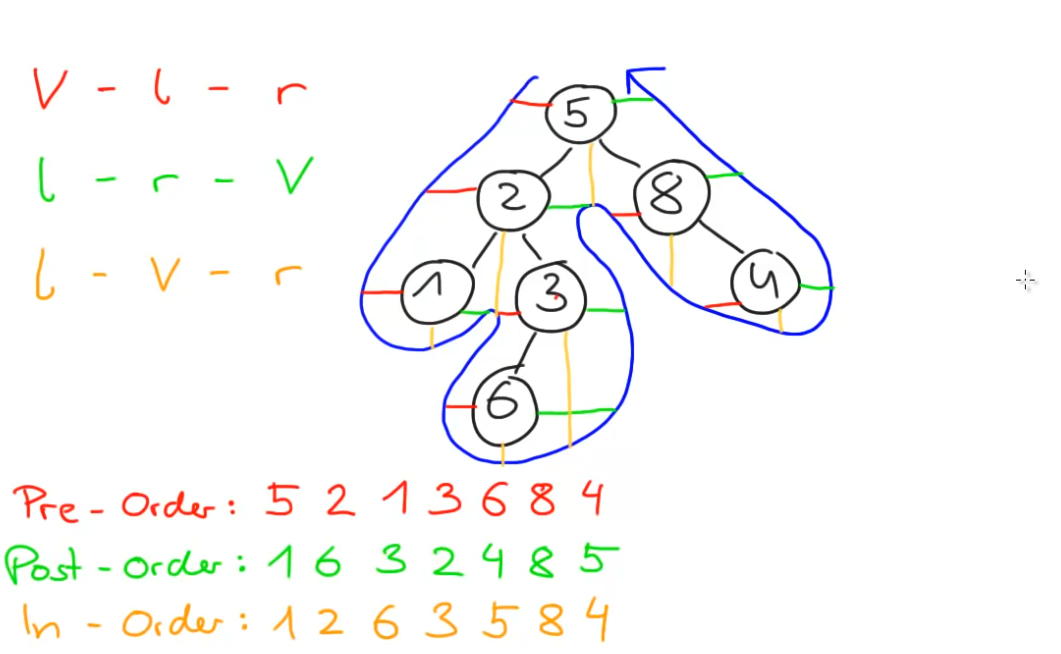
\includegraphics[width=\textwidth,keepaspectratio]{snapshot.png}

\subsubsection*{Löschen von Elementen in Binärbäumen}
\begin{enumerate}
    \item Blatt: Setze das entsprechende Kind des Elternknotens auf null
    \item Halbblatt: Ersetze den zu löschenden Knoten durch sein Kind
    \item Elternknoten: Ersetze den Wert des Knotens durch seinen In-Order-Nachbar 
            (der größte Knoten des linken Teilbaums oder der kleinste des rechten)
\end{enumerate}

\section*{Laufzeit}
Die Laufzeit eines Programs wird mithilfe der O ("oh") Notation, auch Landau Notation genannt, abgeschätzt.
Sie gibt an, wie die Ausführzeit eines Programs mit wachsender Problemgröße wächst.
Die Laufzeiten sind (in steigender Komplexität)
\begin{itemize}
    \item Konstant (1,2,1000)
    \item Logarithmisch ($\log_2 n; \log_3 n$)
    \item Linear (3n, n, 1000n)
    \item Linearithmisch ($n \log_2 n; n \log_6 n$)
    \item Polinomial ($n^2;n^4$)
    \item Exponential ($2^n;4^n$)
\end{itemize}
Achtung! $\log_2 n$ wächst schneller als $\log_6 n$

\section*{Rekursion}
Rekusive Funktionen sind Funktionen, die sich selbst aufrufen. Rekursive Lösungen sind
elegant, haben jedoch häufig längere Laufzeiten als ihre iterativen Equivalente. Jedes
rekursive Programm kann auch iterativ implementiert werden. Rekursive Funktionen haben 
immer eine \emph{Abbruchbedingung}, ohne die sie sich unendlich oft selbst aufrufen würden.

Die Laufzeit einer rekuriven Funktion, die sich selbst mehrfach aufruft ist immer exponentiell.
Dies lässt sich im Rekursionsbaum ablesen. Vervielfacht sich der Baum bei jedem Schritt so ist
die Laufzeit exponentiell.
\end{document}